\chapter{From Ising Magnets to Liquid--Gas Criticality}

\lectureoverview{The liquid--gas transition can be reached by an unexpected route. We first complete the mean-field treatment of the Ising magnet, identify its coexistence line and critical point, and then reinterpret an up spin as an occupied lattice site. The resulting lattice gas has hard-core exclusion, short-range attraction, a chemical potential controlled by the magnetic field, and precisely the same phase diagram. The formal course concludes with critical behavior and universality. A separate postlecture discussion then examines what physicists mean by fine-tuning, how selection effects can enter an explanation, and why such reasoning is useful only when joined to a mechanism and possible tests.}

\section{Why Boiling Water Begins with a Magnet}

Boiling water is the familiar phenomenon we would like to understand: a liquid changes into a gas and its density changes abruptly. The standard route passes through the van der Waals equation. Here we take a different route. We return to the Ising magnet, finish its mean-field description, and then discover that the same model can be read as a fluid.

This is more than a picturesque analogy. Once the variables have been translated correctly, the Ising magnet and the lattice gas are the same statistical-mechanical system. Magnetization becomes particle density, the external magnetic field becomes a chemical potential, and the magnetic coexistence line becomes the liquid--gas coexistence line. The translation explains why two apparently different pieces of matter can have the same critical behavior.

Mean field will not supply exact numerical answers in low dimension. In one dimension it even predicts a transition that the exact solution forbids. Its value here is structural. In two and three dimensions it reveals the right order parameter, the competing phases, the critical endpoint, and the way an infinitesimal bias selects one phase. In three dimensions, where every site has six nearest neighbors, replacing those neighbors by their average already gives a useful qualitative picture.

\section{The Ising Energy Bookkeeping}

Put a two-state spin on every site of a hypercubic lattice,
\begin{equation}
\sigma_i=\pm1.
\end{equation}
We use the Hamiltonian
\begin{equation}
\mathcal H
=-J\sum_{\langle ij\rangle}\sigma_i\sigma_j
+h\sum_i\sigma_i,
\qquad J>0.
\label{eq:ising-hamiltonian}
\end{equation}
The notation matters. The first sum is over nearest-neighbor \emph{links}; the second is over \emph{sites}. A link is counted once, not once from each endpoint.

For a single link,
\begin{equation}
E_{ij}=-J\sigma_i\sigma_j.
\end{equation}
Parallel spins have energy \(-J\), while antiparallel spins have energy \(+J\). A broken bond therefore costs
\begin{equation}
\Delta E_{\rm bond}=+J-(-J)=2J.
\label{eq:broken-bond}
\end{equation}
The number \(2J\), rather than either absolute link energy, is what controls the relative Boltzmann weights. We could add a constant to every configuration without changing any probability.

\begin{classroomqa}
\audiencequestion{Why are there two different sums in the Hamiltonian?}
\lecturerresponse{The exchange energy belongs to a pair of neighboring sites, so it is summed over links \(\langle ij\rangle\). The field acts independently on each spin, so it is summed over sites \(i\). Confusing those two countings introduces exactly the factors of two that will matter in mean field. \lecturetimestamp{00:08:04--00:08:45}}
\end{classroomqa}

\begin{classroomqa}
\audiencequestion{Does making \(J\) larger simply make every energy more negative?}
\lecturerresponse{It enlarges the separation between aligned and misaligned configurations. The zero of energy is arbitrary; the physical statement is that a broken bond costs \(2J\). Larger positive \(J\) therefore makes thermal disorder less favorable at a fixed temperature. \lecturetimestamp{00:08:47--00:10:17}}
\end{classroomqa}

On an infinite or periodic hypercubic lattice in \(d\) dimensions, every site has \(2d\) neighbors. Counting from all \(N\) sites counts every link twice, so
\begin{equation}
N_{\rm links}=\frac{(2d)N}{2}=dN.
\label{eq:number-links}
\end{equation}
An aligned configuration consequently has exchange energy \(-JdN\). Boundary sites alter this by a surface term, negligible compared with \(N\) in the thermodynamic limit. The two completely aligned states are degenerate when \(h=0\).

The field term fixes a sign convention that we shall keep consistently. In equation~\eqref{eq:ising-hamiltonian}, positive \(h\) gives the lower site energy to \(\sigma=-1\). Thus \(h>0\) favors negative magnetization, while \(h<0\) favors positive magnetization. One can reverse this convention by writing \(-h\sum_i\sigma_i\); nothing physical changes, but every later sign must then be reversed with it.

\begin{classroomqa}
\audiencequestion{Where does temperature enter if the Hamiltonian contains only \(J\) and \(h\)?}
\lecturerresponse{Temperature enters through the Boltzmann factor \(e^{-\beta\mathcal H}\), with \(\beta=1/T\) in units \(k_{\rm B}=1\). The dimensionless quantities are therefore \(\beta J\) and \(\beta h\). \lecturetimestamp{00:13:07--00:13:43}}
\end{classroomqa}

\section{One Spin in the Average Field of Its Neighbors}

Choose a spin far from the boundary. It has \(2d\) nearest neighbors. Mean field replaces each fluctuating neighbor by the same average
\begin{equation}
m=\expect{\sigma}.
\end{equation}
The exchange energy involving the chosen spin \(\sigma\) is then
\begin{equation}
-J\sigma\sum_{\text{\(2d\) neighbors}}\sigma_j
\;\longrightarrow\;-2dJm\,\sigma.
\end{equation}
Adding the external field gives the effective one-spin energy
\begin{equation}
\mathcal H_{\rm mf}(\sigma)=(-2dJm+h)\sigma.
\label{eq:mean-field-one-spin}
\end{equation}
The factor \(2d\) is essential. It is easy to omit while writing the central-spin picture, and it was restored explicitly during the board derivation.

\begin{figure}[ht]
\centering

\includegraphics[width=0.84\textwidth]{lecture_10_figure_02.png}
\caption{A central spin surrounded by its mean-field neighbors, together with the one-spin energy and the developing self-consistency equation.}
\lectureframe{00:17:57}
\end{figure}

The one-spin partition function is
\begin{align}
z_{\rm mf}
&=\sum_{\sigma=\pm1}
\exp\!\left[-\beta(-2dJm+h)\sigma\right] \\
&=2\cosh\!\left[\beta(2dJm-h)\right].
\end{align}
Its average spin is
\begin{align}
\expect{\sigma}
&=\frac{\sum_{\sigma=\pm1}\sigma
 e^{\beta(2dJm-h)\sigma}}
{\sum_{\sigma=\pm1}e^{\beta(2dJm-h)\sigma}} \\
&=\tanh\!\left[\beta(2dJm-h)\right].
\end{align}
But the spin we selected is supposed to be typical of the neighbors whose average we called \(m\). Self-consistency therefore requires
\begin{equation}
\boxed{m=\tanh\!\left[\beta(2dJm-h)\right].}
\label{eq:mean-field-self-consistency}
\end{equation}
This one nonlinear equation is the mean-field reduction of the many-spin problem.

\begin{classroomqa}
\audiencequestion{Why is the average on the left the same \(m\) that was inserted for every neighbor?}
\lecturerresponse{That equality is the approximation. We assume a homogeneous bulk state, replace the actual environment by its average, calculate the central spin in that environment, and demand that the calculated average reproduce the environment we assumed. A solution is a self-consistent bulk state. \lecturetimestamp{00:16:28--00:18:00}}
\end{classroomqa}

Introduce
\begin{equation}
y=2\beta dJm.
\label{eq:y-definition}
\end{equation}
Since \(\beta=1/T\),
\begin{equation}
m=\frac{yT}{2dJ},
\end{equation}
and equation~\eqref{eq:mean-field-self-consistency} becomes
\begin{equation}
\boxed{\frac{yT}{2dJ}=\tanh(y-\beta h).}
\label{eq:reduced-mean-field}
\end{equation}

\begin{figure}[ht]
\centering

\includegraphics[width=0.82\textwidth]{lecture_10_figure_03.png}
\caption{The reduced self-consistency equation after introducing \(y=2\beta dJm\), ready to be solved graphically.}
\lectureframe{00:24:42}
\end{figure}

\begin{classroomqa}
\audiencequestion{Why does the field appear as \(y-\beta h\), and which spin does a positive field favor?}
\lecturerresponse{Our Hamiltonian contains \(+h\sigma\). Its Boltzmann exponent is therefore \(\beta(2dJm-h)\sigma\), so the hyperbolic tangent contains \(y-\beta h\). Positive \(h\) favors \(\sigma=-1\). If one instead defines the Hamiltonian with \(-h\sigma\), every occurrence of \(h\) changes sign and the phase diagram is reflected horizontally. \lecturetimestamp{00:18:17--00:20:00}}
\end{classroomqa}

\section{Graphical Solutions and the Curie Point}

Set \(h=0\). We must find the intersections of
\begin{equation}
\frac{T}{2dJ}y
\qquad\text{and}\qquad
\tanh y.
\end{equation}
The first is a straight line through the origin; the second is an odd, saturating curve. At high temperature the line is steep and the only intersection is \(y=0\), hence \(m=0\). As the temperature falls, the line becomes shallower. The critical temperature is reached when the line and the hyperbolic tangent are tangent at the origin.

\begin{figure}[ht]
\centering
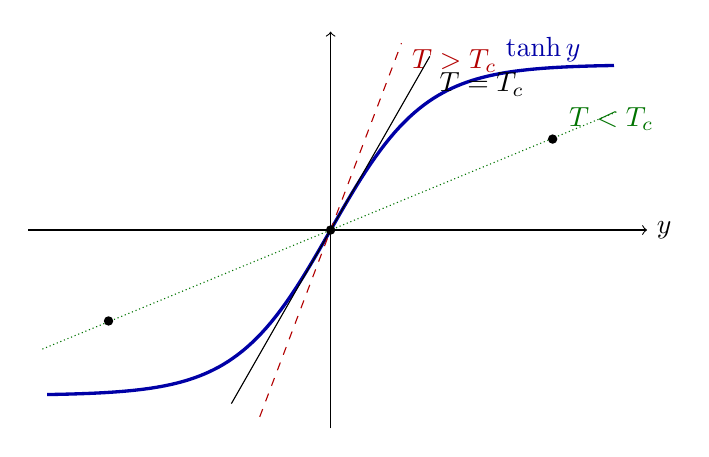
\begin{tikzpicture}[x=1.2cm,y=2.1cm]
\draw[->] (-3.2,0) -- (3.35,0) node[right] {$y$};
\draw[->] (0,-1.2) -- (0,1.2);
\draw[very thick,blue!65!black,domain=-3:3,samples=120]
  plot (\x,{tanh(\x)});
\node[blue!65!black,above] at (2.25,0.96) {$\tanh y$};
\draw[dashed,red!70!black] (-0.75,-1.13) -- (0.75,1.13);
\node[red!70!black,right] at (0.76,1.02) {$T>T_c$};
\draw[black] (-1.05,-1.05) -- (1.05,1.05);
\node[right] at (1.05,0.88) {$T=T_c$};
\draw[densely dotted,green!45!black] (-3.05,-0.72) -- (3.05,0.72);
\node[green!45!black,right] at (2.42,0.67) {$T<T_c$};
\fill (-2.35,-0.55) circle (1.7pt);
\fill (0,0) circle (1.7pt);
\fill (2.35,0.55) circle (1.7pt);
\end{tikzpicture}
\caption{The mean-field equation at zero field. Below \(T_c\), the two nonzero intersections represent the stable magnetized phases; the zero solution remains algebraically present but is unstable.}
\label{fig:mean-field-intersections}
\end{figure}

Because
\begin{equation}
\left.\frac{d}{dy}\tanh y\right|_{y=0}=1,
\end{equation}
the tangency condition is
\begin{equation}
\frac{T_c}{2dJ}=1.
\end{equation}
Thus mean field predicts
\begin{equation}
\boxed{T_c^{\rm MF}=2dJ.}
\label{eq:mean-field-tc}
\end{equation}
Below this temperature there are two stable nonzero solutions \(\pm m_0(T)\). The solution \(m=0\) still satisfies the equation, but it is no longer a stable equilibrium. The system chooses one of the two symmetry-related magnetized phases.

\begin{classroomqa}
\audiencequestion{Is this the Curie temperature?}
\lecturerresponse{Yes. For a ferromagnet the temperature at which spontaneous magnetization disappears is conventionally called the Curie temperature. Here \(2dJ\) is its mean-field value, not an exact low-dimensional result. \lecturetimestamp{00:28:19--00:28:57}}
\end{classroomqa}

Near the transition, expand the hyperbolic tangent:
\begin{equation}
\tanh y=y-\frac{y^3}{3}+O(y^5).
\end{equation}
At \(h=0\), equation~\eqref{eq:reduced-mean-field} gives
\begin{equation}
\left(1-\frac{T}{T_c}\right)y-\frac{y^3}{3}+O(y^5)=0.
\end{equation}
The nonzero branches therefore behave as
\begin{equation}
y^2\simeq3\left(1-\frac{T}{T_c}\right),
\qquad
m\propto(T_c-T)^{1/2}.
\label{eq:mf-beta-exponent}
\end{equation}
The square root is a mean-field critical exponent. Its precise value will not survive in low dimension, but the continuous vanishing of the order parameter at the endpoint will.

\section{The Temperature--Field Plane and Branch Selection}

The material fixes \(J\); the experimenter can vary \(T\) and \(h\). It is therefore natural to draw a phase diagram in the \(T\)--\(h\) plane. Below \(T_c\), an arbitrarily small field selects one of the two magnetized branches. With our convention, \(h<0\) selects \(m>0\), while \(h>0\) selects \(m<0\).

At zero temperature the spins are fully aligned, so \(m=\pm1\). At high temperature the zero-field average is \(m=0\). As the critical point is approached along \(h=0\), the magnitude \(m_0(T)\) falls continuously to zero. But at any fixed \(T<T_c\), crossing \(h=0\) switches discontinuously from \(+m_0(T)\) to \(-m_0(T)\).

\begin{figure}[ht]
\centering

\includegraphics[width=0.90\textwidth]{lecture_10_figure_06.png}
\caption{The coexistence line in the \(T\)--\(h\) plane and the magnetization branches at fixed temperature below \(T_c\).}
\lectureframe{00:39:30}
\end{figure}

\begin{figure}[ht]
\centering
\begin{tikzpicture}[x=1.25cm,y=1.15cm]
\begin{scope}
\draw[->] (-2.45,0) -- (2.55,0) node[right] {$h$};
\draw[->] (0,0) -- (0,3.7) node[above] {$T$};
\draw[very thick,red!70!black] (0,0) -- (0,2.35);
\fill[red!70!black] (0,2.35) circle (2.3pt);
\node[right] at (0.08,2.35) {$T_c$};
\node at (-1.25,1.05) {$m>0$};
\node at (1.25,1.05) {$m<0$};
\draw[->,rounded corners,blue!65!black] (-1.65,0.85) -- (-1.65,3.02)
 -- (1.65,3.02) -- (1.65,0.85);
\node[blue!65!black] at (0,3.35) {continuous path};
\end{scope}
\begin{scope}[xshift=7.0cm,yshift=1.55cm]
\draw[->] (-2.5,0) -- (2.5,0) node[right] {$h$};
\draw[->] (0,-1.35) -- (0,1.4) node[above] {$m$};
\draw[very thick,blue!65!black]
  (-2.2,1.05) .. controls (-0.75,1.03) and (-0.2,0.75) .. (-0.08,0.62);
\draw[very thick,blue!65!black]
  (0.08,-0.62) .. controls (0.2,-0.75) and (0.75,-1.03) .. (2.2,-1.05);
\draw[dashed] (0,0.62) -- (0,-0.62);
\fill (0,0.62) circle (1.8pt);
\fill (0,-0.62) circle (1.8pt);
\node at (0,-1.75) {\(T<T_c\)};
\end{scope}
\end{tikzpicture}
\caption{At fixed \(T<T_c\), magnetization jumps across the coexistence line. In the full two-parameter plane, the two phases can instead be connected continuously by going around the critical point.}
\label{fig:ising-phase-plane}
\end{figure}

\begin{classroomqa}
\audiencequestion{What happens if the field is exactly zero below \(T_c\)?}
\lecturerresponse{The ideal infinite system has two equally good pure phases. Any infinitesimal residual bias, boundary condition, or fluctuation associated with preparation selects one of them. The thermodynamic discontinuity is expressed by the two one-sided limits \(m(T,0^-)=+m_0(T)\) and \(m(T,0^+)=-m_0(T)\) in our sign convention. \lecturetimestamp{00:35:04--00:37:10}}
\end{classroomqa}

\begin{classroomqa}
\audiencequestion{Is this the same thing as hysteresis?}
\lecturerresponse{Hysteresis concerns metastability and the history-dependent delay with which a real system switches branches. It is related, but it requires dynamics beyond the equilibrium phase diagram and is not developed here. \lecturetimestamp{00:37:11--00:37:20}}
\end{classroomqa}

\begin{classroomqa}
\audiencequestion{Can the positive and negative phases be connected without crossing a discontinuity?}
\lecturerresponse{Yes. Raise the temperature above \(T_c\), change the sign of the field there, and lower the temperature again. That path goes around the endpoint and the magnetization changes continuously. The jump is unavoidable only when one crosses \(h=0\) at fixed \(T<T_c\). \lecturetimestamp{00:37:20--00:38:15}}
\end{classroomqa}

\begin{classroomqa}
\audiencequestion{Does the magnetization approach zero whenever \(h\) approaches zero?}
\lecturerresponse{Not at a generic temperature below \(T_c\). There the one-sided limits are nonzero. The spontaneous magnetization approaches zero only as the critical temperature itself is approached. \lecturetimestamp{00:38:29--00:39:45}}
\end{classroomqa}

\section{A Permeable Box and the Chemical Potential}

We now leave magnets and begin again with particles. Imagine a region whose potential energy is lower than that of the surrounding space. The walls are permeable: particles can enter and leave. If the interior energy is lower by an amount \(\mu\), occupation inside receives a relative Boltzmann factor \(e^{\beta\mu}\). Deepening or raising the well changes the average number of particles in the box.

\begin{figure}[ht]
\centering

\includegraphics[width=0.84\textwidth]{lecture_10_figure_07.png}
\caption{The potential-well picture of a permeable box. The energy difference between inside and outside controls the preference for particles to occupy the box.}
\lectureframe{00:41:30}
\end{figure}

\begin{figure}[ht]
\centering
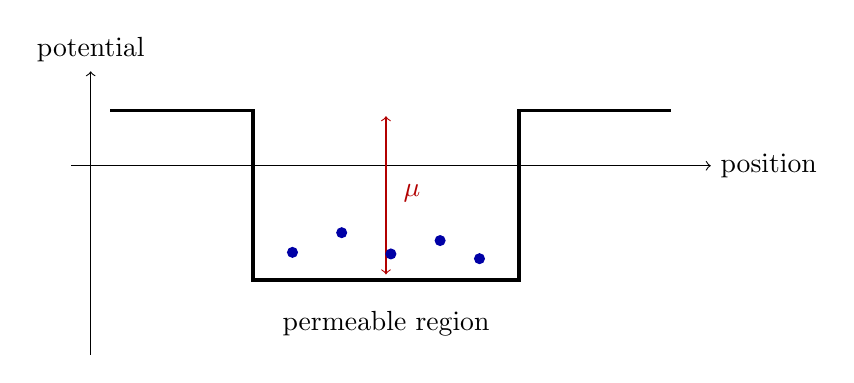
\begin{tikzpicture}[x=1.25cm,y=1.0cm]
\draw[->] (-3.2,0) -- (3.3,0) node[right] {position};
\draw[->] (-3.0,-2.4) -- (-3.0,1.2) node[above] {potential};
\draw[very thick] (-2.8,0.7) -- (-1.35,0.7)
 -- (-1.35,-1.45) -- (1.35,-1.45) -- (1.35,0.7) -- (2.9,0.7);
\draw[<->,red!70!black] (0,0.63) -- (0,-1.38);
\node[right,red!70!black] at (0.08,-0.35) {$\mu$};
\foreach \x/\y in {-0.95/-1.1,-0.45/-0.85,0.05/-1.12,0.55/-0.95,0.95/-1.18}
  \fill[blue!65!black] (\x,\y) circle (2pt);
\node at (0,-2.0) {permeable region};
\end{tikzpicture}
\caption{Changing the potential offset changes the particle-number preference. In a grand-canonical description, that offset is represented by the chemical potential.}
\end{figure}

This thought experiment makes chemical potential concrete. It is an energy advantage per added particle relative to a reservoir. If several species can pass through the wall, each species has its own chemical potential. A sealed box is different: then \(N\) is fixed and the chemical potential is inferred thermodynamically rather than imposed by exchange with a reservoir.

\begin{classroomqa}
\audiencequestion{Is the depth of the well literally the chemical potential?}
\lecturerresponse{It is a direct mechanical realization of a chemical-potential difference. Lowering every one-particle level inside by \(\mu\) contributes \(-\mu N\) to the energy and therefore \(+\beta\mu N\) to the Boltzmann exponent. Only differences of chemical potential matter. \lecturetimestamp{00:44:49--00:45:40}}
\end{classroomqa}

Because particles may enter and leave, the partition sum must include all particle numbers:
\begin{equation}
\Xi(T,\mu)
=\sum_{N=0}^{\infty}\;\sum_{\mathcal C_N}
\exp\!\left[-\beta E(\mathcal C_N)+\beta\mu N\right].
\label{eq:grand-partition}
\end{equation}
The inner sum runs over configurations with a specified \(N\); the outer sum runs over \(N\) itself. The grand-canonical weight may also be written \(e^{-\beta(E-\mu N)}\).

\begin{figure}[ht]
\centering

\includegraphics[width=0.88\textwidth]{lecture_10_figure_08.png}
\caption{The permeable box and the grand-canonical sum over particle number and configurations.}
\lectureframe{00:47:15}
\end{figure}

\begin{classroomqa}
\audiencequestion{What changes when the box is sealed?}
\lecturerresponse{The particle number stops fluctuating. One then uses the canonical partition function at fixed \(N\). In the permeable box, \(N\) is a thermodynamic variable controlled on average by \(\mu\). \lecturetimestamp{00:45:42--00:47:50}}
\end{classroomqa}

At fixed temperature, varying \(\mu\) ordinarily changes the density smoothly. Below a critical temperature it can instead cause an abrupt jump. That is the fluid phenomenon we are seeking. To obtain it microscopically, the particles need two features: they must not be able to occupy the same place, and they must attract at short range.

\section{Turning Spins into a Lattice Gas}

Keep the lattice but reinterpret its two states. Define an occupation number
\begin{equation}
n_i=\frac{1+\sigma_i}{2}
=
\begin{cases}
0,&\sigma_i=-1,\\
1,&\sigma_i=+1.
\end{cases}
\label{eq:occupation-map}
\end{equation}
An empty site has spin down; an occupied site has spin up. Because \(n_i\) can only be zero or one, double occupancy is forbidden. The lattice itself therefore supplies the hard core.

\begin{figure}[ht]
\centering

\includegraphics[width=0.84\textwidth]{lecture_10_figure_04.png}
\caption{The lattice-gas identification begins with \(\sigma=-1\) as an empty site; \(\sigma=+1\) is then an occupied site.}
\lectureframe{00:53:45}
\end{figure}

Begin with the empty lattice, all \(\sigma=-1\). Every bond is aligned and has energy \(-J\). That constant vacuum energy can be subtracted. Now place one particle on a site in two dimensions. The corresponding spin flips to \(+1\), breaking four bonds. Each broken bond costs \(2J\), so
\begin{equation}
\Delta E_1=4(2J)=8J.
\label{eq:one-particle-cost}
\end{equation}
Two particles far apart break eight bonds and cost \(16J\). If the two particles occupy neighboring sites, the bond between them is aligned again. Only six boundary bonds are broken, and the cost is
\begin{equation}
\Delta E_{2,\rm adjacent}=6(2J)=12J.
\end{equation}
Bringing the particles together therefore lowers the energy by
\begin{equation}
16J-12J=4J.
\label{eq:lattice-attraction}
\end{equation}
The live count was first described as a \(2J\) saving and then corrected: one shared link removes two broken-boundary contributions, so the attraction is \(4J\).

\begin{figure}[ht]
\centering

\includegraphics[width=0.84\textwidth]{lecture_10_figure_05.png}
\caption{The two-dimensional bond count: one isolated particle costs \(8J\), two distant particles cost \(16J\), and two adjacent particles cost \(12J\).}
\lectureframe{01:00:25}
\end{figure}

The lattice gas now has both required molecular properties. The binary occupation supplies hard-core exclusion, and the exchange interaction supplies a nearest-neighbor attraction of strength \(4J\). The particle number is allowed to fluctuate because spin flips change the number of occupied sites.

\subsection{The exact algebraic dictionary}

The bond-counting picture is enough to see the physics, but the exact change of variables makes the equivalence unmistakable. Substitute
\begin{equation}
\sigma_i=2n_i-1
\end{equation}
into equation~\eqref{eq:ising-hamiltonian}. For a link,
\begin{equation}
\sigma_i\sigma_j
=4n_in_j-2n_i-2n_j+1.
\end{equation}
On a regular \(d\)-dimensional lattice,
\begin{equation}
\sum_{\langle ij\rangle}(n_i+n_j)=2d\sum_i n_i.
\end{equation}
Therefore
\begin{align}
\mathcal H
&=-4J\sum_{\langle ij\rangle}n_in_j
+(4dJ+2h)\sum_i n_i+\text{constant}.
\label{eq:ising-as-lattice-gas}
\end{align}
Compare this with the conventional lattice-gas Hamiltonian
\begin{equation}
\mathcal H_{\rm lg}
=-\epsilon\sum_{\langle ij\rangle}n_in_j
-\mu\sum_i n_i+\text{constant}.
\label{eq:lattice-gas-hamiltonian}
\end{equation}
The dictionary is
\begin{equation}
\boxed{\epsilon=4J,\qquad
\mu=-(4dJ+2h).}
\label{eq:chemical-potential-map}
\end{equation}

\begin{figure}[ht]
\centering

\includegraphics[width=0.88\textwidth]{lecture_10_figure_09.png}
\caption{The exchange and field terms beside the particle-energy count. The field changes the insertion energy without changing the nearest-neighbor attraction.}
\lectureframe{01:04:30}
\end{figure}

In two dimensions, an isolated insertion changes the energy by
\begin{equation}
8J+2h=-\mu.
\end{equation}
The \(8J\) comes from broken bonds; \(2h\) comes from changing one spin from \(-1\) to \(+1\). Adjusting \(h\) therefore adjusts the chemical potential while leaving the attraction \(4J\) fixed. The field is not literally equal to \(\mu\), because the exchange baseline contributes the offset \(4dJ\).

\begin{classroomqa}
\audiencequestion{If the field controls particle number, why is \(h\) not simply the chemical potential?}
\lecturerresponse{Creating a particle also breaks exchange bonds relative to the empty reference state. The conventional coefficient of \(-N\) is therefore \(\mu=-(4dJ+2h)\), not merely \(-2h\). The offset depends on \(J\) and the coordination number. \lecturetimestamp{01:06:28--01:06:41}}
\end{classroomqa}

The density is equally simple:
\begin{equation}
\rho=\expect{n_i}
=\frac{1+\expect{\sigma_i}}{2}
=\frac{1+m}{2}.
\label{eq:density-map}
\end{equation}
Thus \(m=-1\) is the empty lattice, \(m=+1\) is the completely filled lattice, and \(m=0\) is half filling. The total particle number is \(N_{\rm p}=\sum_i n_i\); the density is \(N_{\rm p}/N\).

\begin{figure}[ht]
\centering

\includegraphics[width=0.90\textwidth]{lecture_10_figure_10.png}
\caption{The density relation \(\rho=(1+m)/2\) written beside the magnetic coexistence line.}
\lectureframe{01:08:25}
\end{figure}

\begin{classroomqa}
\audiencequestion{Is \((1+m)/2\) the number of particles or the density?}
\lecturerresponse{It is the mean occupation per site, hence the dimensionless lattice density. Multiplying by the total number of sites gives the expected particle number. The distinction between an intensive density and an extensive count is important. \lecturetimestamp{01:06:43--01:09:31}}
\end{classroomqa}

\section{The Magnetic Phase Diagram Becomes the Fluid Phase Diagram}

Translate figure~\ref{fig:ising-phase-plane} using equations~\eqref{eq:chemical-potential-map} and \eqref{eq:density-map}. Above \(T_c\), changing \(\mu\) changes the density smoothly. Below \(T_c\), crossing the coexistence value
\begin{equation}
\mu_{\rm coex}=-4dJ
\qquad(h=0)
\label{eq:coexistence-mu}
\end{equation}
causes the density to jump between a dilute gas and a dense liquid. At \(T_c\) the two densities merge and the discontinuity disappears.

\begin{figure}[ht]
\centering

\includegraphics[width=0.92\textwidth]{lecture_10_figure_11.png}
\caption{The Ising coexistence line read as a liquid--gas phase diagram. The gas lies on the low-density side, the liquid on the high-density side, and the two can be connected continuously around the critical endpoint.}
\lectureframe{01:14:30}
\end{figure}

\begin{figure}[ht]
\centering
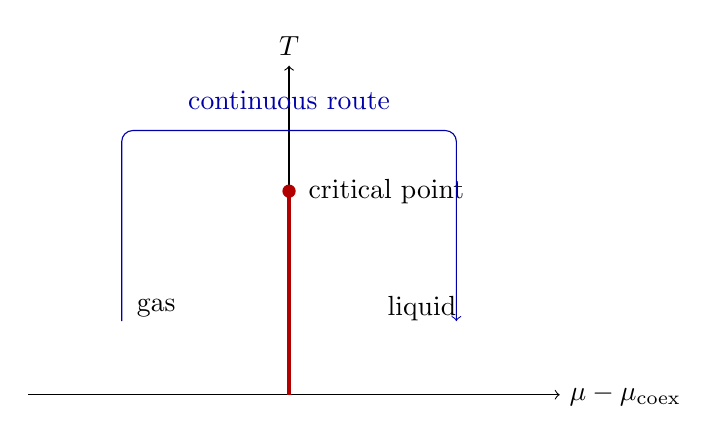
\begin{tikzpicture}[x=1.25cm,y=1.1cm]
\draw[->] (-2.65,0) -- (2.75,0) node[right] {$\mu-\mu_{\rm coex}$};
\draw[->] (0,0) -- (0,3.8) node[above] {$T$};
\draw[very thick,red!70!black] (0,0) -- (0,2.35);
\fill[red!70!black] (0,2.35) circle (2.4pt);
\node[right] at (0.1,2.35) {critical point};
\node at (-1.35,1.0) {gas};
\node at (1.35,1.0) {liquid};
\draw[->,blue!65!black,rounded corners]
 (-1.7,0.85) -- (-1.7,3.05) -- (1.7,3.05) -- (1.7,0.85);
\node[blue!65!black] at (0,3.4) {continuous route};
\end{tikzpicture}
\caption{The liquid and gas are distinct phases below the endpoint, yet no singular boundary separates them in the supercritical region.}
\label{fig:liquid-gas-plane}
\end{figure}

This identifies the familiar boiling line. At a fixed pressure, heating a liquid until it crosses coexistence produces boiling. At fixed temperature, changing pressure or chemical potential can cross the same boundary. A superheated vapor or supercooled liquid is a metastable continuation beyond equilibrium coexistence; describing its lifetime requires nucleation dynamics, which lie beyond this equilibrium construction.

\begin{classroomqa}
\audiencequestion{Is superheated steam represented in this phase diagram?}
\lecturerresponse{The equilibrium diagram identifies the coexistence boundary. A superheated or supersaturated state is metastable: it persists temporarily on the wrong side because forming a critical droplet has an interfacial free-energy cost. That kinetic refinement is not calculated here. \lecturetimestamp{01:12:19--01:12:29}}
\end{classroomqa}

\begin{classroomqa}
\audiencequestion{How does one vary chemical potential in an ordinary fluid?}
\lecturerresponse{The potential-well box is the clean theoretical control. In the laboratory one more often changes pressure, volume, or contact with a reservoir; thermodynamics then translates those controls into a change of chemical potential. \lecturetimestamp{01:12:30--01:13:59}}
\end{classroomqa}

\begin{classroomqa}
\audiencequestion{When the density changes, are we changing the molecular potential \(J\)?}
\lecturerresponse{No. For a fixed substance, \(J\) represents the short-range attraction and remains fixed in this model. Changing \(\mu\) changes how many sites are occupied and therefore the distribution of intermolecular separations. Changing \(J\) would mean changing the microscopic substance or interaction. \lecturetimestamp{01:14:50--01:15:41}}
\end{classroomqa}

\begin{classroomqa}
\audiencequestion{Is the critical temperature the same thing as the ordinary boiling point?}
\lecturerresponse{No. A boiling point is specified at a chosen pressure, so it moves along the coexistence curve when the pressure changes. The critical temperature is the unique endpoint above which liquid and gas are no longer separated by a phase boundary. Pressure has not been derived explicitly in this lattice-gas treatment. \lecturetimestamp{01:15:42--01:17:02}}
\end{classroomqa}

One can now state the central result. The Ising magnet and the lattice gas do not merely draw similar diagrams. They share a partition function after a change of variables and parameters. Every singular thermodynamic property on one side has a counterpart on the other:
\begin{equation}
\begin{array}{c|c}
\text{Ising magnet} & \text{lattice gas}\\ \hline
\sigma_i=\pm1 & n_i=0,1\\
m=\expect{\sigma} & \rho=(1+m)/2\\
h & \mu=-(4dJ+2h)\\
\text{aligned exchange} & \text{nearest-neighbor attraction}\\
h=0,\ T<T_c & \text{liquid--gas coexistence}\\
(T_c,0) & \text{critical endpoint}
\end{array}
\label{eq:ising-fluid-dictionary}
\end{equation}

\section{Critical Exponents and Universality}

Close to a critical point, thermodynamic quantities often develop power-law singularities. With reduced temperature
\begin{equation}
t=\frac{T-T_c}{T_c},
\end{equation}
one writes, schematically,
\begin{equation}
m\sim(-t)^{\beta_{\rm crit}},
\qquad
\chi\sim |t|^{-\gamma},
\qquad
\xi\sim |t|^{-\nu}.
\label{eq:critical-exponents}
\end{equation}
Here \(\beta_{\rm crit}\) is a critical exponent, not inverse temperature. Mean field gives \(\beta_{\rm crit}=1/2\), but fluctuations change the exponents below the upper critical dimension.

The exponents need not be integers. They need not all be irrational either: the two-dimensional Ising model famously has several exact rational exponents, whereas the three-dimensional Ising values are nontrivial numbers determined with high precision by theory and computation. The robust lesson is that the exponents are generally not fixed by elementary dimensional analysis.

Even more strikingly, microscopic details often do not fix them. Systems with the same spatial dimension, the same order-parameter symmetry, and sufficiently short-range interactions can flow to the same long-distance critical theory. They belong to one \emph{universality class}. A uniaxial magnet and an ordinary liquid--gas endpoint both have a single scalar order parameter and share the Ising universality class in the same dimension.

\begin{classroomqa}
\audiencequestion{Are universality classes a finite or discrete list?}
\lecturerresponse{There are many classes, organized by dimension, symmetries, conservation laws, interaction range, and other long-distance data. In many familiar cases the fixed points and exponent sets are discrete, but there are also systems with continuously varying exponents. The safe claim is not that the catalog is finite; it is that many microscopically different systems share the same long-distance data. \lecturetimestamp{01:18:50--01:19:38}}
\end{classroomqa}

\begin{classroomqa}
\audiencequestion{If liquid and gas coexist, what separates them in an actual container?}
\lecturerresponse{An interface does. Surface tension penalizes interfacial area, while gravity creates a vertical chemical-potential gradient and usually places the denser liquid below the gas. In negligible gravity the geometry is controlled more directly by surface tension and boundary conditions. \lecturetimestamp{01:19:40--01:21:18}}
\end{classroomqa}

\begin{classroomqa}
\audiencequestion{Where is the heat of vaporization in this picture?}
\lecturerresponse{Below the critical point, crossing the first-order coexistence line generally carries latent heat. The heat of vaporization tends to zero as the critical endpoint is approached because the two phases become identical there. This lecture establishes the phase structure but does not calculate the latent heat. \lecturetimestamp{01:21:19--01:22:18}}
\end{classroomqa}

\begin{classroomqa}
\audiencequestion{Can a phase transition be used as a sensitive detector, for example with a superconducting device?}
\lecturerresponse{Yes. Near a transition, a small perturbation can produce a large response or trigger a change of state. Practical detectors exploit that sensitivity, although the relevant order parameter and dynamics may differ from the Ising example. \lecturetimestamp{01:22:19--01:24:05}}
\end{classroomqa}

This completes the statistical-mechanics course. The route began with entropy and equilibrium, passed through partition functions and gases, and ended by showing that a magnet and a fluid can be two descriptions of the same critical phenomenon.

\section{Postlecture Discussion: Fine-Tuning and Selection}

After the formal lecture ended, the conversation continued for roughly forty minutes. It is worth preserving, but it should not be confused with the derivation above. The subject is no longer the lattice gas. It is the logic of fine-tuning and the cautious use of anthropic selection in cosmology.

\subsection{Small numbers are not automatically fine-tuned}

There is no single sentence that settles every use of the phrase \emph{anthropic principle}. The useful starting point is operational: when a theory permits many realized environments, observations are conditioned on the fact that observers can arise only in some of them. That conditional statement can be rational. It becomes empty if invoked without an ensemble, a selection condition, or a mechanism that makes the alternatives physically meaningful.

Before selection enters, one must distinguish a small parameter from a fine-tuned parameter. A number can be small because a stable dynamical mechanism drives it to a special value. Fine-tuning means that the observed value appears to require an extraordinarily precise balance among otherwise independent contributions, with no known restoring mechanism or symmetry protecting the balance.

\begin{classroomqa}
\audiencequestion{Can the anthropic principle be stated sharply?}
\lecturerresponse{Its defensible use is conditional rather than mystical: if many physically realized environments have different parameters, then the environments observed by beings like us are drawn from the subset compatible with observers. That does not by itself generate the environments or assign their probabilities; those tasks belong to the underlying physics. \lecturetimestamp{01:25:45--01:26:13}}
\end{classroomqa}

The cosmological constant is the motivating example. Its observed magnitude is extraordinarily small compared with naive quantum-field-theory contributions to vacuum energy. The difficulty is not merely that the final number is small. It is that many large terms appear to have to cancel to tremendous accuracy, while no accepted low-energy feedback mechanism adjusts the result toward the observed value.

\subsection{The blimp and the submarine}

Two buoyancy examples isolate the distinction. A blimp floats at an altitude where its average density matches the density of the surrounding air. Air density decreases with height. If the blimp rises, the external air becomes less dense and the blimp tends to descend; if it falls, the external air becomes denser and the blimp tends to rise. The density match may be numerically delicate, but the atmospheric gradient provides restoring feedback. The equilibrium is dynamically explained.

A neutrally buoyant submarine in nearly incompressible water is different. Water density changes little with depth. If the submarine's average density happens to equal the surrounding water, no comparable depth-dependent restoring mechanism explains that equality. A tiny mismatch makes it rise or sink. Achieving neutral buoyancy requires precise adjustment of ballast and contents. The small residual is then a fine-tuning unless some control system or design mechanism accounts for it.

\begin{figure}[ht]
\centering
\begin{tikzpicture}[>=Latex]
\begin{scope}[xshift=-3.8cm]
\shade[top color=blue!5,bottom color=blue!28] (-2.5,-2.2) rectangle (2.5,2.2);
\draw[very thick,rounded corners=18pt,fill=yellow!35]
  (-1.15,0) ellipse (1.15 and 0.55);
\draw[thick] (0,-0.55) -- (0,-1.05);
\draw[thick,fill=gray!20] (-0.45,-1.05) rectangle (0.45,-1.38);
\draw[->,red!70!black,thick] (1.65,1.45) -- (1.65,0.55)
 node[midway,right] {restoring};
\draw[->,red!70!black,thick] (-1.65,-1.45) -- (-1.65,-0.55)
 node[midway,left] {restoring};
\node at (0,2.55) {\textbf{Blimp: density gradient}};
\node[align=center] at (0,-2.75) {displacement changes\\the buoyant imbalance};
\end{scope}
\begin{scope}[xshift=3.8cm]
\shade[top color=cyan!10,bottom color=blue!45] (-2.5,-2.2) rectangle (2.5,2.2);
\draw[very thick,fill=gray!35,rounded corners=12pt]
  (-1.45,-0.25) -- (1.1,-0.25) arc (-90:90:0.38)
  -- (-1.45,0.51) -- cycle;
\draw[thick] (-0.25,0.51) -- (-0.25,0.85) -- (0.35,0.85) -- (0.35,0.51);
\draw[->,red!70!black,thick] (1.65,0.15) -- (1.65,1.35)
 node[midway,right] {rise};
\draw[->,red!70!black,thick] (-1.65,0.15) -- (-1.65,-1.35)
 node[midway,left] {sink};
\node at (0,2.55) {\textbf{Submarine: nearly uniform density}};
\node[align=center] at (0,-2.75) {no depth-dependent feedback\\protects neutral buoyancy};
\end{scope}
\end{tikzpicture}
\caption{A small residual can be dynamically stable or genuinely tuned. The blimp has restoring feedback; the idealized submarine requires its average density to be adjusted to the water.}
\label{fig:blimp-submarine}
\end{figure}

\begin{classroomqa}
\audiencequestion{Why should the submarine crew demand an explanation if neutral buoyancy is observed?}
\lecturerresponse{Because, absent a ballast-control mechanism, neither a symmetry nor environmental feedback protects the equality of two independent densities. The question is not whether the equality is logically possible, but why the system occupies such a narrow region of its parameter space. \lecturetimestamp{01:35:05--01:36:25}}
\end{classroomqa}

\subsection{Many domains and conditional observation}

Now imagine a process that produces an enormous number of submarines with many different average densities. Most sink or rise; only a tiny fraction remain for long periods in the habitable band between surface and bottom. An observer who necessarily lives in one of the surviving submarines should not be surprised to measure near-neutral buoyancy. The observation is selected by the condition required for the observer to be present.

This reasoning needs two ingredients:
\begin{enumerate}
\item a physical process that actually realizes many alternatives, rather than alternatives that exist only in imagination;
\item a selection condition explaining why observations are made only in a restricted subset.
\end{enumerate}
Selection does not replace the production mechanism. It changes the conditional probability of what an observer measures once the ensemble exists.

\begin{classroomqa}
\audiencequestion{Is the argument merely that unlikely things happen somewhere in a sufficiently large sample?}
\lecturerresponse{That is only the first half. The second is observational conditioning: the observers are not sampled uniformly from all domains but only from domains where their existence is possible. A complete proposal still needs a measure over domains and a physical account of how they are produced. \lecturetimestamp{01:39:19--01:40:36}}
\end{classroomqa}

Applied to vacuum energy, a large negative cosmological constant can make a universe recollapse too rapidly, while a sufficiently large positive value can prevent matter from condensing into galaxies. The observed value lies in the narrow range compatible with long-lived structure. This provides a possible selection condition, not a derivation of the distribution of cosmological constants.

Quantum field theory adds the fine-tuning problem: vacuum contributions from different fields and scales are individually much larger than the observed residual. If those terms cancel almost exactly, the result resembles the carefully balanced submarine rather than the self-correcting blimp. The analogy is meant to expose the logical problem, not to supply its solution.

\begin{classroomqa}
\audiencequestion{Could changes in one parameter be compensated by changes in several others?}
\lecturerresponse{Yes. The viable set need not be a narrow interval on one axis; it may be a thin surface in a multidimensional parameter space. Correlated changes can preserve structure, but the question then becomes why the realized parameters lie near that surface and what measure the underlying theory assigns to it. \lecturetimestamp{01:45:10--01:46:19}}
\end{classroomqa}

\begin{figure}[ht]
\centering
\begin{tikzpicture}[x=1.3cm,y=1.05cm,>=Latex]
\draw[->] (-3.2,0) -- (3.4,0) node[right] {$\lambda_1$};
\draw[->] (0,-2.5) -- (0,2.65) node[above] {$\lambda_2$};
\fill[gray!12] (-3,-2.25) rectangle (3.1,2.3);
\draw[very thick,blue!65!black]
 (-2.8,-1.55) .. controls (-1.3,-0.75) and (0.15,0.05) .. (2.85,1.55);
\draw[very thick,blue!25]
 (-2.8,-1.25) .. controls (-1.3,-0.45) and (0.15,0.35) .. (2.85,1.85);
\fill[blue!15,opacity=.65]
 (-2.8,-1.55) .. controls (-1.3,-0.75) and (0.15,0.05) .. (2.85,1.55)
 -- (2.85,1.85) .. controls (0.15,0.35) and (-1.3,-0.45) .. (-2.8,-1.25) -- cycle;
\node[blue!65!black,rotate=28] at (1.3,0.95) {viable band};
\foreach \x/\y in {-2.4/1.45,-1.7/-1.8,-0.9/1.8,0.3/-1.45,1.2/1.85,2.4/-0.8}
  \fill[red!65!black] (\x,\y) circle (2pt);
\fill[green!45!black] (0.55,0.58) circle (2.8pt);
\node[green!35!black,right] at (0.65,0.55) {observed domain};
\end{tikzpicture}
\caption{With several parameters, habitability or structural viability may occupy a thin correlated band rather than a narrow interval of one parameter. Selection constrains observations to the band but does not generate the parameter distribution.}
\label{fig:viable-parameter-band}
\end{figure}

\subsection{Landscape proposals and their uncertainties}

One proposed source of alternatives is a theory with many metastable vacua, possibly populated in different cosmological domains. String-theory landscape ideas and eternal-inflation scenarios are examples, but their detailed realization and probability measure remain uncertain. The lecture presents this as a possibility, not an established fact.

Symmetry would be a more conventional explanation if it forced the cosmological constant to vanish exactly. The difficulty is that the observed accelerated expansion corresponds to a small nonzero value. A mechanism that naturally gives exactly zero does not automatically explain a tiny residual; breaking the symmetry can simply reintroduce the tuning. The submarine image returns here: a rope could hold it at a chosen depth, but then the rope is the mechanism that must be identified rather than assumed.

\begin{classroomqa}
\audiencequestion{Does measuring a parameter very precisely violate the uncertainty principle?}
\lecturerresponse{No. An uncertainty relation applies to specified pairs of noncommuting observables. A coupling constant or vacuum parameter can have a sharply defined value without being the canonical conjugate of an uncontrolled observable. Precision by itself is not an uncertainty-principle paradox. \lecturetimestamp{01:49:21--01:49:36}}
\end{classroomqa}

\begin{classroomqa}
\audiencequestion{Does anthropic reasoning explain the value, or merely restate that observers require it?}
\lecturerresponse{Selection alone is not a dynamical explanation. Its legitimate role is to alter conditional probabilities in a physically realized ensemble. Used without an ensemble, a measure, or testable consequences, it risks becoming a label rather than an explanation. \lecturetimestamp{01:49:37--01:50:21}}
\end{classroomqa}

\subsection{Moderate coincidences in particle physics}

Not every life-relevant parameter is tuned to the same extraordinary degree. Familiar matter depends on photons, electrons, light quarks, and the strong interaction; neutrinos influence cosmology but are not the direct binding agents of atoms. The proton--neutron mass difference is particularly consequential. Because the neutron is slightly heavier than the proton, isolated neutrons can decay and ordinary hydrogen is stable. Reversing the ordering by enough would radically alter nuclear chemistry.

The electron mass and the fine-structure constant likewise set atomic sizes and binding energies. Changing them substantially would change chemistry. These are meaningful sensitivity statements, but they should not be inflated into a claim that every small variation forbids every conceivable form of complexity. Compared with the cosmological-constant problem, many such coincidences are moderate and correlated with other parameters.

The hierarchy associated with the electroweak scale is another prominent naturalness problem: radiative contributions tend to make a fundamental scalar mass sensitive to high scales unless protected by additional structure. Its status and interpretation differ from the vacuum-energy problem, and neither should be reduced to a slogan.

\begin{classroomqa}
\audiencequestion{Would changing the proton--neutron mass difference really matter for ordinary matter?}
\lecturerresponse{Yes. The observed ordering permits stable hydrogen and controls beta stability across nuclei. Modest changes can reorganize nuclear abundances and stellar burning. A careful analysis must vary the coupled parameters consistently rather than changing one number while freezing all the rest. \lecturetimestamp{01:51:47--01:53:08}}
\end{classroomqa}

\begin{classroomqa}
\audiencequestion{What roles do the electron mass and fine-structure constant play?}
\lecturerresponse{They set characteristic atomic energy and length scales, schematically \(E_{\rm atom}\sim \alpha^2m_e\) and \(a_0\sim(\alpha m_e)^{-1}\) in units \(\hbar=c=1\). Large changes would reshape chemistry, although the exact viable region is a multidimensional question. \lecturetimestamp{01:53:09--01:54:12}}
\end{classroomqa}

\subsection{Disagreement, time dependence, and tests}

The discussion briefly turns to criticism of inflation and to the interpretation of precision cosmological data. That historical disagreement should be represented as disagreement, not settled by rhetoric. Inflation has successful phenomenological predictions and many model variants; questions about initial conditions, measures, and testability remain active. Data constrain models, but no single conversational reference to an experiment settles the whole framework.

\begin{classroomqa}
\audiencequestion{Could the cosmological constant vary slowly with time instead of being constant?}
\lecturerresponse{A dynamical dark-energy field can produce time-dependent acceleration. It introduces a potential and initial conditions that must themselves be explained, and observations constrain the equation of state to be close to a cosmological constant. In the lecture-era discussion, no evidence required appreciable time variation. \lecturetimestamp{01:57:17--01:59:19}}
\end{classroomqa}

\begin{classroomqa}
\audiencequestion{Does anthropic selection itself nucleate different universes or domains?}
\lecturerresponse{No. Selection says which realized domains can contain observers; it does not create the domains. A separate cosmological mechanism, such as vacuum transitions during an inflationary history, would have to generate them. \lecturetimestamp{01:59:20--01:59:42}}
\end{classroomqa}

The causal order must remain clear:
\begin{equation}
\text{laws and initial conditions}
\longrightarrow
\text{physical environments}
\longrightarrow
\text{observers and observations}.
\end{equation}
Observers do not reach backward and dictate the laws. Conditioning enters when we ask what an observer drawn from the realized environments is likely to measure.

The scientific question is therefore not whether the language sounds philosophical, political, or religious. It is whether the proposal has a defined physical ensemble, a computable or at least constrained measure, and consequences that could distinguish it from alternatives. Possible signatures discussed for multivacuum cosmology include traces of collisions between bubble domains. Such signals are difficult to predict robustly and none had been established in the cosmic microwave background in the lecture-era discussion. Absence of an easy test is a serious limitation, not a license either to declare the idea true or to dismiss the underlying fine-tuning problem.

\begin{classroomqa}
\audiencequestion{What would turn this from a selection argument into a scientific theory?}
\lecturerresponse{The proposal needs a mechanism that generates the alternatives, a probability measure or controlled substitute, and observable consequences. Bubble-collision signatures are one possible avenue, but their absence or ambiguity illustrates how demanding the testability problem is. \lecturetimestamp{02:02:31--02:04:12}}
\end{classroomqa}

The postlecture exchange ends on that disciplined note. Fine-tuning is evidence that an explanation may be missing. Symmetry, dynamical adjustment, and environmental selection are logically different candidate explanations. Selection can be rational, but only as one component of a physical account whose assumptions and limits are stated openly.
